\section{Redes Neurais Recorrentes}
\label{s.rnn}

\begin{frame}{Redes Neurais Recorrentes}
	\begin{itemize}
		\justifying
		\item Elman~\cite{Elman:90} propôs as Redes Neurais Recorrentes, do inglês \emph{Recurrent Neural Networks} (RNN);
		\\~\\
		\item Pertencem à uma categoria de redes em que a conexão entre seus nós forma um \textbf{grafo direcionado} ao longo de uma sequência;
	\end{itemize}
\end{frame}

\begin{frame}
	\begin{figure}[!ht]
		\centering
		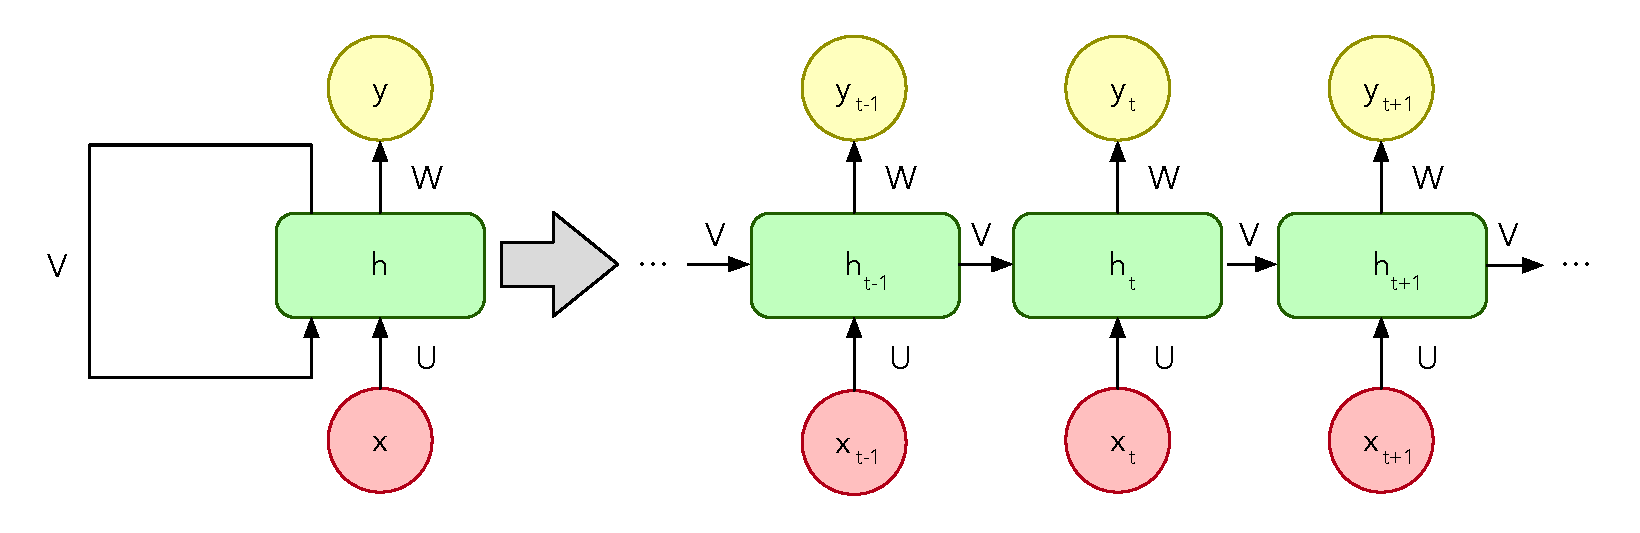
\includegraphics[scale=0.4]{figs/rnn.eps}	
		\label{f.rnn}
		\caption{Arquitetura básica de uma Rede Neural Recorrente.}
	\end{figure}
\end{frame}

\begin{frame}
	\begin{itemize}
		\justifying
		\item Utilização do fator tempo durante o treinamento pode acarretar no problema da \textbf{dissipação do gradiente};
		\\~\\
		\item Gradiente torna-se extremamente \textbf{pequeno} ao longo das iterações, prevenindo as atualizações de pesos;
		\\~\\
		\item Alternativa está na arquitetura em profundidade da \textbf{Rede de Memória de Longo Prazo}.
	\end{itemize}
\end{frame}

\subsection{Rede de Memória de Longo Prazo}
\label{ss.lstm}

\begin{frame}{Rede de Memória de Longo Prazo}
	\begin{itemize}
		\justifying
		\item Hochreiter et al.~\cite{Hochreiter:97} propuseram as Redes de Memória de Longo Prazo, do inglês \emph{Long Short-Term Memory} (LSTM);
		\\~\\
		\item Tipo especial de RNNs, explicitamente projetadas para aprenderem informações por \textbf{longos períodos} de tempo.
	\end{itemize}
\end{frame}

\begin{frame}
	\begin{figure}[!ht]
		\centering
		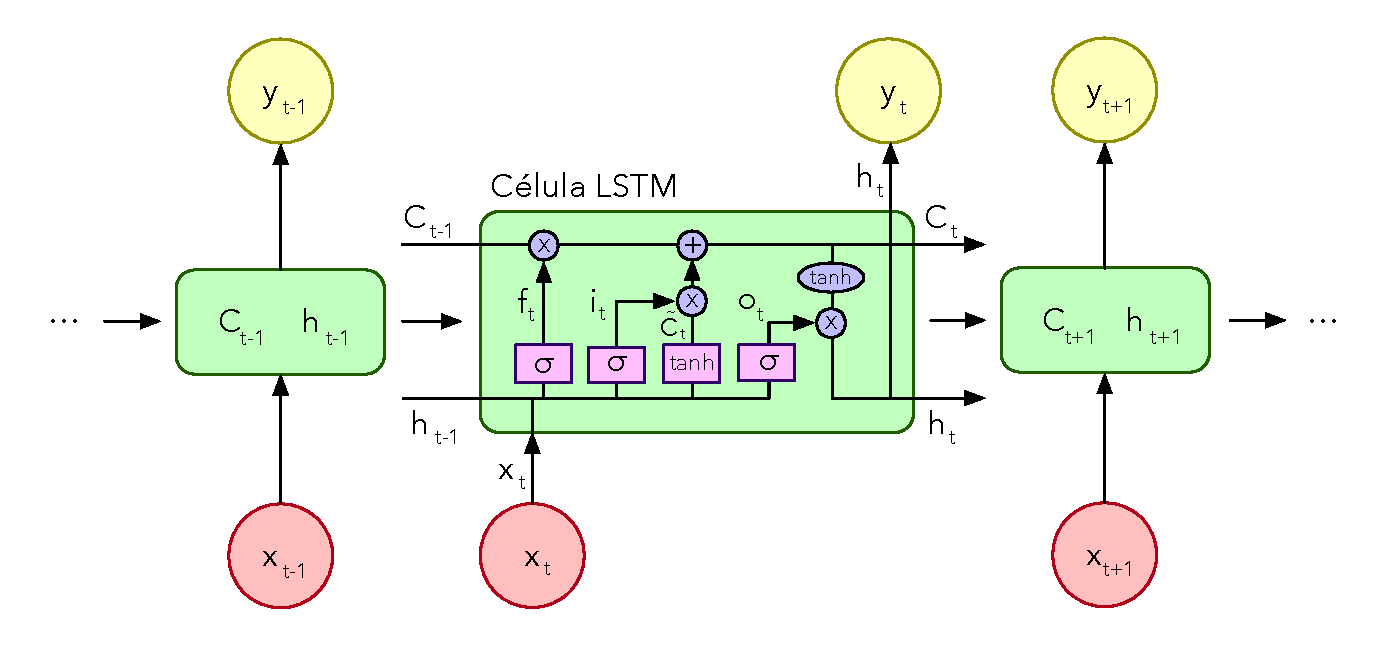
\includegraphics[scale=0.4]{figs/lstm.eps}	
		\label{f.lstm}
		\caption{Arquitetura de uma célula de uma Rede de Memória de Longo Prazo.}
	\end{figure}
\end{frame}

\subsection{Unidade Recorrente de Porta}
\label{ss.gru}

\begin{frame}{Unidade Recorrente de Porta}
	\begin{itemize}
		\justifying
		\item Cho et al.~\cite{Cho:14} introduziram as Unidades Recorrentes de Porta, do inglês \emph{Gated Recurrent Units} (GRU);
		\\~\\
		\item Também procuram solucionar o problema da dissipação ou estouro do gradiente e são vistas como variações das LSTMs.	
	\end{itemize}
\end{frame}

\begin{frame}
	\begin{figure}[!ht]
		\centering
		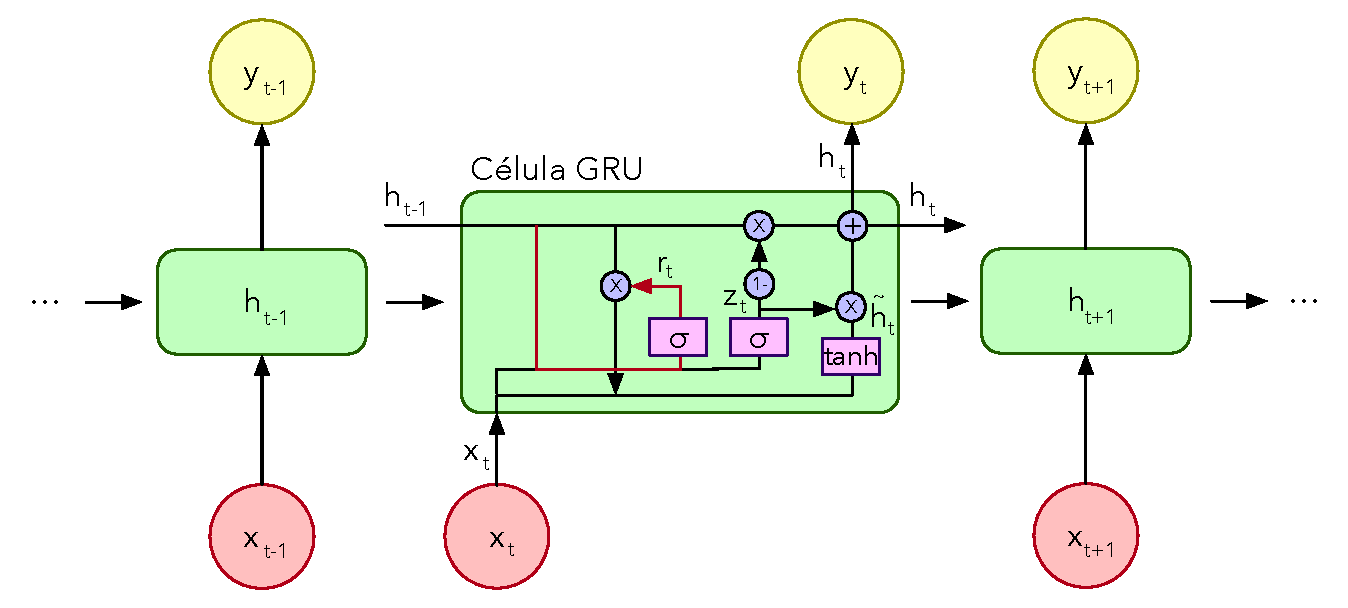
\includegraphics[scale=0.4]{figs/gru.eps}	
		\label{f.gru}
		\caption{Arquitetura de uma Unidade Recorrente de Porta.}
	\end{figure}
\end{frame}